% Source - https://tex.stackexchange.com/a/738063

\documentclass[tikz,border=5pt]{standalone}
\usetikzlibrary{patterns,nfold}
\makeatletter
\tikzset{
  remove inside/.code={%
    \tikzset{even odd rule}%
    \tikz@addmode{\pgfsyssoftpath@getcurrentpath\tikz@temp
      \pgfoffsetpath\tikz@temp{#1}}}}
\makeatother
\tikzset{
    EDR/.style ={
        line width=+1pt,
        preaction={remove inside=#13mm, fill=white},%<-add `fill=white' as preaction 
        preaction={remove inside=#13mm, pattern=north west lines, pattern color=black!75}
    }
}

\begin{document}

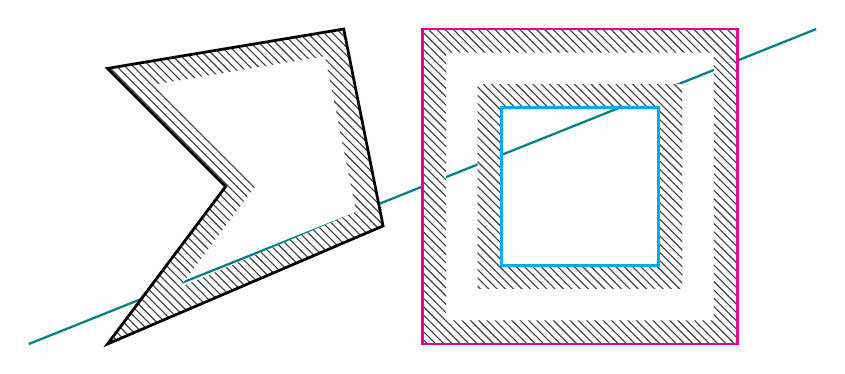
\begin{tikzpicture}
\draw[thick,teal] (0,0) -- (10,4);
\draw[EDR] (1,0) -- (4.5,1.5) -- (4,4) -- (1,3.5) -- (2.5,2) -- cycle;
\draw[magenta,EDR=-] (5,0) rectangle (9,4) ;
\draw[cyan,EDR] (6,1) rectangle (8,3);
\end{tikzpicture}

\end{document}
